\documentclass[11pt]{extarticle}
\usepackage{fullpage,amsmath,amsfonts,microtype,nicefrac,amssymb, amsthm}
\usepackage[left=1in, bottom=1in, top=1in, right = 1in]{geometry}
\usepackage{textcomp}
\usepackage{mathpazo}
\usepackage{mathrsfs}
\usepackage[T1]{fontenc}
\usepackage[utf8]{inputenc}
\usepackage[english]{babel}
\usepackage{graphicx}

\usepackage{microtype}

\usepackage{bm}
\usepackage{dsfont}
\usepackage{enumerate}
\usepackage{ragged2e}

\setlength{\parindent}{24pt}
\setlength{\jot}{8pt}


\usepackage[shortlabels]{enumitem}


%% FOOTNOTES
\usepackage[bottom]{footmisc}
\usepackage{footnotebackref}


%% FIGURE ENVIRONMENT
%\graphicspath{{}}
\usepackage[margin=15pt, font=small, labelfont={bf}, labelsep=period]{caption}
\usepackage{subcaption}
\captionsetup[figure]{name={Figure}, position=above}
\usepackage{float}
\usepackage{epstopdf}


%% NEW COMMANDS
\renewcommand{\baselinestretch}{1.25} 
\renewcommand{\qedsymbol}{$\blacksquare$}
\newcommand{\R}{\mathbb{R}}
\newcommand{\indep}{\mathrel{\text{\scalebox{1.07}{$\perp\mkern-10mu\perp$}}}}
\renewcommand{\b}{\begin}
\newcommand{\e}{\end}

%% NEWTHEOREM
\theoremstyle{plain}
\newtheorem{thm}{Theorem}
\newtheorem{lem}[thm]{Lemma}
\newtheorem{prop}[thm]{Proposition}

\theoremstyle{definition}
\newtheorem{defn}[thm]{Definition}
\newtheorem{ex}[thm]{Example}
\newtheorem{remark}[thm]{Remark}
\newtheorem{cor}[thm]{Corollary}

%% LINKS and COLORS
\usepackage[dvipsnames]{xcolor}
\usepackage{hyperref}
\definecolor{myred}{RGB}{163, 32, 45}
\hypersetup{
	%backref=true,
	%pagebackref=true,
	colorlinks=true,
	urlcolor=myred,
	citecolor=myred, 
	linktoc=all,     
	linkcolor=myred,
}

%% TABLE OF CONTENTS
\addto\captionsenglish{
	\renewcommand{\contentsname}
	{}% This removes the heading over the table of contents.
}



%%%%%%%%%%%%%%%%%%%%%%%%%%%%%%%%%%%%%%%%%%%%%%%%%%%%%%%%%%%%
%%%%%%%%%%%%%%%%%%%%%%%%%%%%%%%%%%%%%%%%%%%%%%%%%%%%%%%%%%%%
%%%%%%%%%%%%%%%%%%%%%%            END PREAMBLE           %%%%%%%%%%%%%%%%%%%%%%%%
%%%%%%%%%%%%%%%%%%%%%%%%%%%%%%%%%%%%%%%%%%%%%%%%%%%%%%%%%%%%
%%%%%%%%%%%%%%%%%%%%%%%%%%%%%%%%%%%%%%%%%%%%%%%%%%%%%%%%%%%%

\title{Dynamic Optimization: Problem Set \#6}

\author{Andreas Schaab}

\date{Fall, 2022}



\begin{document}

\maketitle
\thispagestyle{empty}
\setcounter{page}{0}


%%%%%%%%%%%%%%%%%%%%%%%%%%%%%%%%%%%%%%%%%%%%%%%%%%%%%%%%%%%%
%%%%%%%%%%%%%%%%%%%%%%%%%%%%%%%%%%%%%%%%%%%%%%%%%%%%%%%%%%%%
\vspace{10mm}
\section*{Problem 1: Going on the job market}

\textbf{Credit: David Laibson} 

Consider the following "job market" optimization problem.
A graduate student works on a project with current market value $x$, where $x$ is an Ito process with drift $\alpha$ and standard deviation $\sigma$ :
$$
d x=\alpha d t+\sigma d z
$$
The student works on the project until she chooses to either (i) take the paper to the job market, generating termination payoff $x$, or (ii) abandon the project and start a new project that has current market value $x=0$. This replacement of projects is made at zero cost. (We assume that the student can only work on one project at a time.)

The optimal policy is a two-sided threshold rule. The student stops when (i) $x \geq M$, or (ii) $x \leq 0$. Here $M$ is an endogenous boundary representing the job $M$ arket. The zero bound follows from the economics of the problem (free substitution).

Assume that time has opportunity cost $w$ (annual wage) and the student has an annual discount rate $\rho$.

\begin{enumerate}[(a)]
\item Show that in the continuation region the HJB satisfies $$\rho V = -w+\alpha V^{\prime}+\left(\sigma^2 / 2\right) V^{\prime \prime}$$

\textbf{Solution:}
In this region, the flow utility is $-w$. And the only state variable of the student's problem is $x$
$$
\begin{aligned}
\rho V &=-w+E d V \\
&=-w+\alpha V^{\prime}+\left(\sigma^2 / 2\right) V^{\prime \prime}
\end{aligned}
$$


\item This is the so-called complete equation. The associated reduced equation is
$$
\left(\sigma^2 / 2\right) V^{\prime \prime}+\alpha V^{\prime}-\rho V=0
$$
Guess the solution of the reduced form is $V=\exp (r x)$ and verify, show there are two solutions.

\textbf{Solution:}
  $$
\begin{aligned}
\left(\sigma^2 / 2\right) r^2 \exp (r x)+\alpha r \exp (r x)-\rho \exp (r x) &=0 \\
\left(\sigma^2 / 2\right) r^2+\alpha r-\rho &=0
\end{aligned}
$$
The two roots that solve the reduced equation are
$$
r^{+,-}=\frac{-\alpha \pm \sqrt{\alpha^2+2 \sigma^2 \rho}}{\sigma^2} .
$$

A particular solution of the complete equation is generated by the policy of never stopping:
$$
V(x)=-w / \rho .
$$
The general solution of the complete equation is:
$$
V(x)=C^{+} \exp \left(r^{+} x\right)+C^{-} \exp \left(r^{-} x\right)-w / \rho
$$
Remember that the superscripts $+$ and $-$ are not arithmetic operators.

\item We have three boundary conditions (one value matching condition and two smooth pasting conditions; why aren't we using the other value matching condition at $0 ?)$.
$$
\begin{aligned}
V(M) &=M \\
V^{\prime}(M) &=1 \\
V^{\prime}(0) &=0
\end{aligned}
$$
Derive the two smooth pasting conditions (with the V'), interpret each of the boundary conditions.

\textbf{Solution:} Using the boundary condition $$(V(M) =M)$$ differentiate w.r.t $x$ and evaluate at $x=M$. For $x=0$, because at this boundary start a new project, the value function does not depend on the current $x$. 

\item  We can now solve for our three free variables:  $C^{+}, C^{-}, M $. Show the solution must satisfy 

$$
\begin{gathered}
C^{-}=-r^{+} C^{+} / r^{-} \\
C^{+}=\frac{1}{r^{+}\left[\exp \left(r^{+} M\right)-\exp \left(r^{-} M\right)\right]} \\
C^{-}=\frac{1}{r^{-}\left[\exp \left(r^{-} M\right)-\exp \left(r^{+} M\right)\right]} \\
M=\frac{r^{+} \exp \left(r^{+} M\right)-r^{-} \exp \left(r^{-} M\right)}{\exp \left(r^{+} M\right)-\exp \left(r^{-} M\right)}-w / \rho \\
C^{+}+C^{-}=\frac{1 / r^{+}-1 / r^{-}}{\exp \left(r^{+} M\right)-\exp \left(r^{-} M\right)}
\end{gathered}
$$

\textbf{Solution:} Using the boundary conditions 

$$
\begin{aligned}
V(M) &=M=C^{+} \exp \left(r^{+} M\right)+C^{-} \exp \left(r^{-} M\right)-w / \rho \\
V^{\prime}(M) &=1=r^{+} C^{+} \exp \left(r^{+} M\right)+r^{-} C^{-} \exp \left(r^{-} M\right) \\
V^{\prime}(0) &=0=r^{+} C^{+}+r^{+} C^{-}
\end{aligned}
$$

After some algebra, we can then get the equations above.


The solution of the value function looks as follows (for parameters $\alpha=1, \sigma=5, w=1$, and $\rho=0.05$)

     \begin{figure}[H]
    \centering
    %\caption{$\rho=0$ (iid)}
    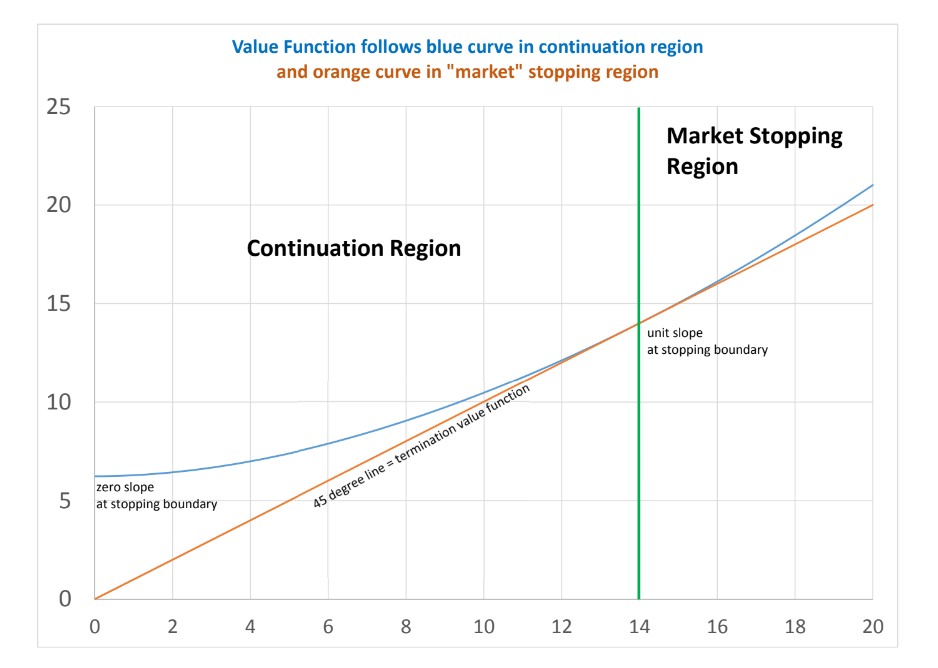
\includegraphics[width=10.2cm]{plot_value_market.png}
    \end{figure}

\item  If you could pick projects with less positive drift (smaller $\alpha$) and more
Brownian noise (larger $\sigma$) would you? Why or why not?

\textbf{Solution:} Depends on parameters. But the main idea is that because only care about getting a very high draw to go on the market, a high  $\sigma$ may maximize the probability of getting into the region $x>M$ fast.  That is, it is a good idea to try risky projects!

\end{enumerate}


%%%%%%%%%%%%%%%%%%%%%%%%%%%%%%%%%%%%%%%%%%%%%%%%%%%%%%%%%%%%
%%%%%%%%%%%%%%%%%%%%%%%%%%%%%%%%%%%%%%%%%%%%%%%%%%%%%%%%%%%%
\vspace{10mm}
\section*{Problem 2: The Equity Premium}

\textbf{Credit: Pablo Kurlat} 

Suppose that consumption growth is:
$$
\frac{c_{t+1}}{c_t}=\left\{\begin{array}{cc}
1+g & \text { with probability } 1-\mu \\
1-D & \text { with probability } \mu
\end{array}\right.
$$
and the (gross) return on the stock market is:
$$
R_{t+1}=\left\{\begin{array}{cc}
1+y & \text { with probability } 1-\mu \\
1-F & \text { with probability } \mu
\end{array}\right.
$$
Furthermore, suppose the event $\frac{c_{t+1}}{c_t}=1-D$ and the event $R_{t+1}=1-F$ always coincide, i.e. $\frac{c_{t+1}}{c_t}$ and $R_t$ are perfectly correlated. The risk-free (gross) real interest rate is $1+r$.
There is a representative household, with preferences given by:
$$
\mathbb{E}\left(\sum_{t=0}^{\infty} \beta^t u\left(c_t\right)\right)
$$
with
$$
u\left(c_t\right)=\frac{c_t^{1-\gamma}}{1-\gamma}
$$

\begin{enumerate}[(a)]
\item Write down the Euler equations for risk-free assets and for the stock market.

\textbf{Solution:} For risk-free assets:
$$
1=\beta(1+r) \mathbb{E}_t\left[\frac{u^{\prime}\left(c_{t+1}\right)}{u^{\prime}\left(c_t\right)}\right]
$$
For the stock market:
$$
1=\beta \mathbb{E}_t\left[\frac{u^{\prime}\left(c_{t+1}\right)}{u^{\prime}\left(c_t\right)}\right] \mathbb{E}_t\left(R_{t+1}\right)+\beta \operatorname{Cov}\left(\frac{u^{\prime}\left(c_{t+1}\right)}{u^{\prime}\left(c_t\right)}, R_{t+1}\right)
$$

\item  Find explicit expressions in terms of parameters for the following quantities:

a) $\mathbb{E}\left(\frac{u^{\prime}\left(c_{t+1}\right)}{u^{\prime}(c t)}\right)$

\textbf{Solution:}
$$
\begin{aligned}
\frac{u^{\prime}\left(c_{t+1}\right)}{u^{\prime}\left(c_t\right)} &=\left(\frac{c_{t+1}}{c_t}\right)^{-\gamma} \\
&=\left\{\begin{array}{cr}
(1+g)^{-\gamma} & \text { with probability } 1-\mu \\
(1-D)^{-\gamma} & \text { with probability } \mu
\end{array}\right.
\end{aligned}
$$
$$
\mathbb{E}\left(\frac{u^{\prime}\left(c_{t+1}\right)}{u^{\prime}\left(c_t\right)}\right)=(1-\mu)(1+g)^{-\gamma}+\mu(1-D)^{-\gamma}
$$

b)$\mathbb{E}\left(R_{t+1}\right)$


\textbf{Solution:} $$
\mathbb{E}\left(R_{t+1}\right)=(1-\mu)(1+y)+\mu(1-F)
$$


c) $Cov\left(\frac{u^{\prime}\left(c_{t+1}\right)}{u^{\prime}\left(c_{t}\right)},R_{t+1}\right)$

\textbf{Solution:} 
$$Cov\left(\frac{u^{\prime}\left(c_{t+1}\right)}{u^{\prime}\left(c_{t}\right)},R_{t+1}\right)=\mathbb{E}\left[\left(\frac{u^{\prime}\left(c_{t+1}\right)}{u^{\prime}\left(c_{t}\right)}-\mathbb{E}\left(\frac{u^{\prime}\left(c_{t+1}\right)}{u^{\prime}\left(c_{t}\right)}\right)\right)\left(R_{t+1}-\mathbb{E}\left(R_{t+1}\right)\right)\right]$$
$$=\left(1-\mu\right)\mathbb{E}\left[\left(\left(1+g\right)^{-\gamma}-\left(1-\mu\right)\left(1+g\right)^{-\gamma}-\mu\left(1-D\right)^{-\gamma}\right)\left(\left(1+y\right)-\left(1-\mu\right)\left(1+y\right)-\mu\left(1-F\right)\right)\right]$$
$$+\mu\mathbb{E}\left[\left(\left(1-D\right)^{-\gamma}-\left(1-\mu\right)\left(1+g\right)^{-\gamma}-\mu\left(1-D\right)^{-\gamma}\right)\left(\left(1-F\right)-\left(1-\mu\right)\left(1+y\right)-\mu\left(1-F\right)\right)\right]$$
$$=\left(1-\mu\right)\mu\left(\left(1+g\right)^{-\gamma}-\left(1-D\right)^{-\gamma}\right)\left(y+F\right)-\mu\left(1-\mu\right)\left(\left(1-D\right)^{-\gamma}-\left(1+g\right)^{-\gamma}\right)\left(y+F\right)$$
$$=2\left(1-\mu\right)\mu\left(y+F\right)\left[\left(1+g\right)^{-\gamma}-\left(1-D\right)^{-\gamma}\right]$$

\item 3. Find an explicit expression in terms of parameters for the value of $\beta$ that is consistent with
the household’s Euler equation for risk-free assets, given that the risk-free rate is $1 + r$.
\textbf{Solution:}
 $$
\begin{aligned}
\beta &=\frac{1}{(1+r) \mathbb{E}_t\left[\frac{u^{\prime}\left(c_{t+1}\right)}{u^{\prime}\left(c_t\right)}\right]} \\
&=\frac{1}{(1+r)\left[(1-\mu)(1+g)^{-\gamma}+\mu(1-D)^{-\gamma}\right]}
\end{aligned}
$$

\item Derive a joint restriction on the values of $\beta, \gamma, \mu, g, D, y$ and $F$ that needs to be satisfied for the household's Euler equation for the stock market to hold.
\textbf{Solution:} 
Using the Euler equation:
$$
\begin{aligned}
1 &=\beta \mathbb{E}_t\left[\frac{u^{\prime}\left(c_{t+1}\right)}{u^{\prime}\left(c_t\right)}\right] \mathbb{E}_t\left(R_{t+1}\right)+\beta \operatorname{Cov}\left(\frac{u^{\prime}\left(c_{t+1}\right)}{u^{\prime}\left(c_t\right)}, R_{t+1}\right) \\
&=\beta\left[(1-\mu)(1+g)^{-\gamma}+\mu(1-D)^{-\gamma}\right][(1-\mu)(1+y)+\mu(1-F)] \\
&+2 \beta(1-\mu) \mu(y+F)\left[(1+g)^{-\gamma}-(1-D)^{-\gamma}\right]
\end{aligned}
$$

\item Set the following parameter values: \\

\begin{tabular}{|c|c|c|c|c|c|}
\hline$r$ & $\gamma$ & $\mu$ & $g$ & $D$ & $F$ \\
\hline $0.01$ & 3 & $0.02$ & $0.015$ & $0.3$ & $0.45$ \\
\hline
\end{tabular}\\

What must be the values of $\beta$ and $y$ for the household's Euler equations to hold?

\textbf{Solution:}
Replacing:
$$
\begin{aligned}
&\beta=0.9946 \\
&y=0.0595
\end{aligned}
$$

\item What is the value of $\mathbb{E}\left(R_{t+1}\right)$ ? What is the equity premium?

\textbf{Solution:} Replacing:
$$
\mathbb{E}\left(R_{l+1}\right)=1.0493
$$
so the premium is
$$
\mathbb{E}\left(R_{t+1}\right)-(1+r)=0.0393
$$

\item Suppose a researcher is trying to measure the equity premium empirically in a sample  the event "$\frac{c_{t+1}}{c_{t}}=1-D$ and $R_{t+1}=1-F$" has never been realized. What would the researcher's estimates be for:

(a) $\mathbb{E}\left(\frac{u^{\prime}\left(c_{t+1}\right)}{u^{\prime}\left(c_t\right)}\right)$

\textbf{Solution:}
$$
\mathbb{E}\left(\frac{u^{\prime}\left(c_{t+1}\right)}{u^{\prime}\left(c_t\right)}\right)=(1+g)^{-\gamma}=0.956
$$
(b) $\mathbb{E}\left(R_{t+1}\right)$

\textbf{Solution:}
$$
\mathbb{E}\left(R_{t+1}\right)=1+y=1.0595
$$
(c) $\operatorname{Cov}\left(\frac{u^{\prime}\left(c_{t+1}\right)}{u^{\prime}\left(c_t\right)}, R_{t+1}\right)$

\textbf{Solution:}
$$
\operatorname{Cov}\left(\frac{u^{\prime}\left(c_{t+1}\right)}{u^{\prime}\left(c_t\right)}, R_{t+1}\right)=0
$$

Would the researcher conclude that there is an equity premium “puzzle”? Explain.
\end{enumerate}


%%%%%%%%%%%%%%%%%%%%%%%%%%%%%%%%%%%%%%%%%%%%%%%%%%%%%%%%%%%%
%%%%%%%%%%%%%%%%%%%%%%%%%%%%%%%%%%%%%%%%%%%%%%%%%%%%%%%%%%%%
\vspace{10mm}
\section*{Problem 3} 

\textbf{Credit:} David Laibson (\url{https://projects.iq.harvard.edu/econ2010c/problem-sets-david-laibson})

Please solve Problem set 4 of David.



%%%%%%%%%%%%%%%%%%%%%%%%%%%%%%%%%%%%%%%%%%%%%%%%%%%%%%%%%%%%
%%%%%%%%%%%%%%%%%%%%%%%%%%%%%%%%%%%%%%%%%%%%%%%%%%%%%%%%%%%%
\vspace{10mm}
\section*{Problem 4} 

\textbf{Credit:} David Laibson (\url{https://projects.iq.harvard.edu/econ2010c/problem-sets-david-laibson})

Please solve Problem 1 of David’s problem set (PSET) \#5.







\end{document}











